\documentclass[11pt]{article}

\usepackage[english]{babel}

\usepackage[a4paper,top=2cm,bottom=2cm,left=1.5cm,right=1.5cm,marginparwidth=1.75cm]{geometry}
\usepackage{multicol}
\usepackage{listings}
\usepackage{amsmath}
\usepackage{booktabs}
\usepackage{caption}
\usepackage{float}  
\usepackage{wrapfig}

\usepackage{graphicx}
\usepackage[colorlinks=true, allcolors=blue]{hyperref}
\usepackage{xcolor}
\definecolor{darkgreen}{rgb}{0,0.5,0}
\DeclareCaptionLabelFormat{bold}{\textbf{#1 #2:}}
\captionsetup[figure]{labelformat=bold}


\lstset{language=Python, 
        basicstyle=\footnotesize\ttfamily,
        keywordstyle=\color{blue},
        commentstyle=\color{darkgreen},
        stringstyle=\color{red},
        showstringspaces=false,
        frame=single}

\title{\huge\bfseries Computational Neuroscience Coursework}
\author{
    \texttt{\Large COMS30017}\\[4ex]
    \bfseries Martin Oravec 2068729
}
\date{December 7, 2023}

\usepackage{titling}
\renewcommand\maketitlehooka{\null\mbox{}\vfill}
\renewcommand\maketitlehookd{\vfill\null}


\hyphenpenalty=10000
\exhyphenpenalty=10000
\sloppy

\begin{document}

\makeatletter
    \begin{titlepage}
        \begin{center}
            
\includegraphics[width=0.35\linewidth]{UoB_Logo.png}\\[40ex]
            {\huge \bfseries  \@title }\\[4ex] 
            {\LARGE  \@author}\\[60ex] 
            {\large \@date}
        \end{center}
    \end{titlepage}
\makeatother
\newpage

\section*{Question 1} \label{question 1}
A Fano factor greater than 1 indicates a distribution with variance greater than its mean, suggesting a degree of variability or dispersion. A Fano factor less than 1 implies a more regular, less variable distribution. The Fano Factor is defined as $F = \frac{\sigma^2}{\mu}$ where \( \sigma^2 \) is the variance of the spike count and \( \mu \) is the mean of the spike count.
A higher coefficient of variation (CV) indicates a higher level of dispersion around the mean, whereas a lower CV indicates less variability in proportion to the mean. The coefficient of variation is defined as $CV = \frac{\sigma}{\mu}$ where \( \sigma \) is the standard deviation of the dataset and \( \mu \) is the mean of the dataset.
Using the following code I generated spikes using the Poisson process.

\begin{lstlisting}[language=Python]
def generate_spike_train(firing_rate, interval, refractory_period=0):
    current_time = 0
    spike_times = []
    
    while current_time < interval:
        if refractory_period > 0 and spike_times:
            current_time += refractory_period
            
        next_spike = np.random.exponential(1 / firing_rate)
        current_time += next_spike
        if current_time < interval:
            spike_times.append(current_time)

    return spike_times
\end{lstlisting}
I used the numpy's random exponential function to correctly model the Poisson process. In a Poisson process, the time intervals between consecutive spikes follow an exponential distribution. This means that the probability of the next spike occurring is independent of the previous spike, known as memorylessness. Here are the results based on an average of 100 simulations of the Fano factor and the coefficient of variation of the inter-spike interval(CV of the ISI).

\begin{figure}[ht]
\begin{minipage}[t]{0.5\textwidth}
\vspace{1mm}
\centering
\textbf{No Refractory Period}
\begin{tabular}{cc}
\toprule
Window Size (s) & Fano factor \\
\midrule
0.01 & 0.999 \\
0.05 & 0.998 \\
0.1  & 1.021 \\
\bottomrule
CV of the ISI: \textbf{1.002}
\end{tabular}
% \vspace{1mm}
\end{minipage}
\begin{minipage}[t]{0.5\textwidth} % Half the text width
\vspace{1mm}
\centering
\textbf{With 5 ms Refractory Period}
\begin{tabular}{cc}
\toprule
Window Size (s) & Fano factor \\
\midrule
0.01 & 0.788 \\
0.05 & 0.745 \\
0.1  & 0.749 \\
\bottomrule
CV of the ISI: \textbf{0.862}\\
\end{tabular}
\vspace{1mm}
\end{minipage}
\caption{Results of the calculated Fano factors and coefficient of variation of the inter-spikes intervals (CV of the ISI) for no refractory period and 5ms refractory period}
\label{fig:results1}
\end{figure}
From these results, the Fano factor of the spike trains generated without the refractory period being roughly equal to 1.0 indicates a Poisson-like distribution where the spike train variability is consistent with a random process. The corresponding CV of ISI was about 1.002, suggesting a high variability of the spike intervals, again aligning with the expectations of a Poisson process. With a 5 ms refractory period the Fano factors are reduced to roughly 0.75, this indicates a decrease in spike count variability as compared to spike trains generated without the refractory period and hence the Poisson model. This is shown also by the CV of the ISI which dropped from 1.0 to about 0.86 reflecting a decrease in the variability of the spike intervals as the effect of the refractory period. This shows the impact on the statistical properties of the generated spike trains when a refractory period is introduced. Further, when we look at the average fire rate of the two with the same fire rate variable, the effective fire rate dropped from roughly 35.0 to 30.0. Collectively, these results demonstrate how the introduction of a refractory period changes the spike train’s characteristics, diverging from the randomness of a Poisson process.

\newpage
\section*{Question 2} \label{question 2}

\begin{wrapfigure}{r}{0.5\textwidth}
    \centering
    \begin{minipage}[t]{0.5\textwidth}
        \vspace{1mm}
        \centering
        \textbf{No Refractory Period}
        \begin{tabular}{cc}
        \toprule
        Window Size (s) & Fano factor \\
        \midrule
        0.01 & 1.098 \\
        0.05 & 2.869 \\
        0.1  & 3.995 \\
        \bottomrule
        CV of the ISI: \textbf{2.001}
        \end{tabular}
        \vspace{1mm}
    \end{minipage}
    \caption{Results for the spikes from the rho.dat file}
    \label{fig:results1}
\end{wrapfigure}
Analysing the data in the provided 'rho.dat' of the neural response of a fly H1 neuron to a white-noise motion stimulus shows the Fano factor values significantly greater than 1.0, indicating a level of variability in spike counts that well surpasses what would be expected from a Poisson process. This shows a more bursty pattern of the spikes and additionally, the coefficient of variation is 2.009 which indicates a substantial irregularity in timings of the spikes. This demonstrates a significantly variable firing pattern with temporal complexity given the external stimuli suggesting it's heavily dependent on those stimuli and responding more to certain patterns which will become more apparent in question 4.

\section*{Question 3} \label{question 3}

To simulate an integrate and fire neuron I created a Python class to decrease the amount of code.

\begin{wrapfigure}{r}{0.65\textwidth}
    \begin{lstlisting}[language=Python]
    class IntegrateAndFireNeuron:
        def __init__(self, 
                     threshold=-55.0, 
                     tau=10.0, 
                     E=-70.0, 
                     absolut_refractory_period=1.0, 
                     relative_refractory_period=4.0, 
                     reset_voltage=-80.0):
            self.threshold = threshold             
            self.tau = tau                         
            self.V = -70.0                         
            self.E = E                            
            self.spikeVol = 20.0                   
            self.restVol = -70.0                   
            self.resetVol = reset_voltage          
            self.timeElapsed = 0.0                 
            self.spikes = []
    
        def step(self, RI, dt):
            self.timeElapsed += dt
            if (self.V == self.spikeVol):
                self.V = self.restVol
    
            dV = dt / self.tau * (self.E - self.V + RI)
            self.V += dV
            if self.V >= self.threshold:
                self.V = 20.0  
                self.spikes.append(self.timeElapsed)
    
            return self.V
    \end{lstlisting}
\end{wrapfigure}

The simulation for the integrate and fire neuron has been done with the following parameters: $V_{t} = -55mV$, $\tau = 10ms$, $R_{m} = 1.0$, $V_{r} = -80mV$. The simulated duration was 10 s with $\delta t$ set to 1ms and continues input $RI = 12mV$. Using the spike train generation from the previous question, while keeping the firing rate of the Poisson process neurons at 35 Hz and no refractory period for better control over the firing rate, I generated a graph for various strengths of the simulated noise/input. In Figure \ref{fig:q3_graph1}, I kept the ratio of inhibitory and excitatory simulated neurons 1 to 1. I also looked at the differences in the simulated frequency of the integrate and fire neurons when changing the ratio of those simulated input neurons.

\begin{figure}[ht]
    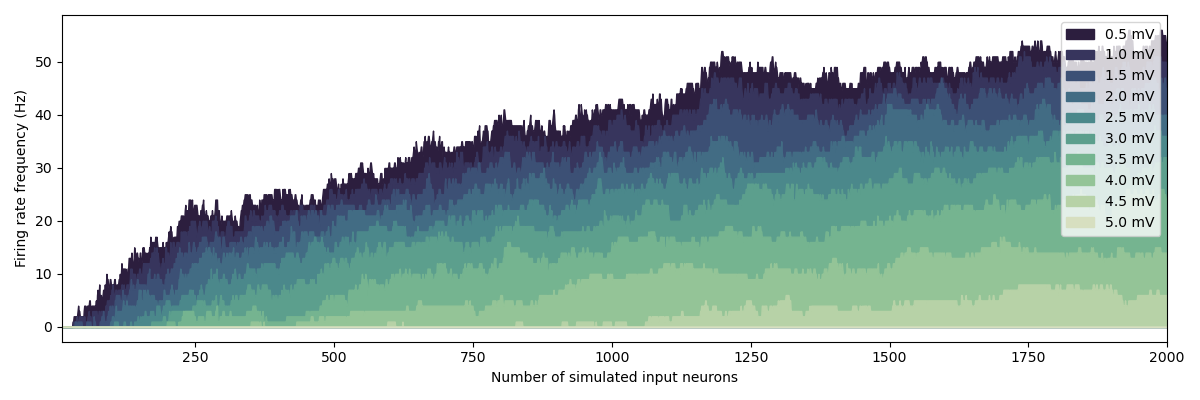
\includegraphics[width=1\linewidth]{Figure_1.png}
    \caption{Integrate and Fire neuron frequencies with a constant input of 10mV and noise input from inhibitory and excitatory Poisson process simulated neurons with various strengths in 1:1 ratio}
    \label{fig:q3_graph1}
\end{figure}

Looking at the graph \ref{fig:q3_graph2} it is apparent that keeping the firing rate frequency of the simulated neuron similar requires more input neurons the lower their input strength becomes. We can look at the Fano factors and coefficients of variations as well that were calculated over a simulated duration of 10 seconds.

\begin{figure}[ht]
    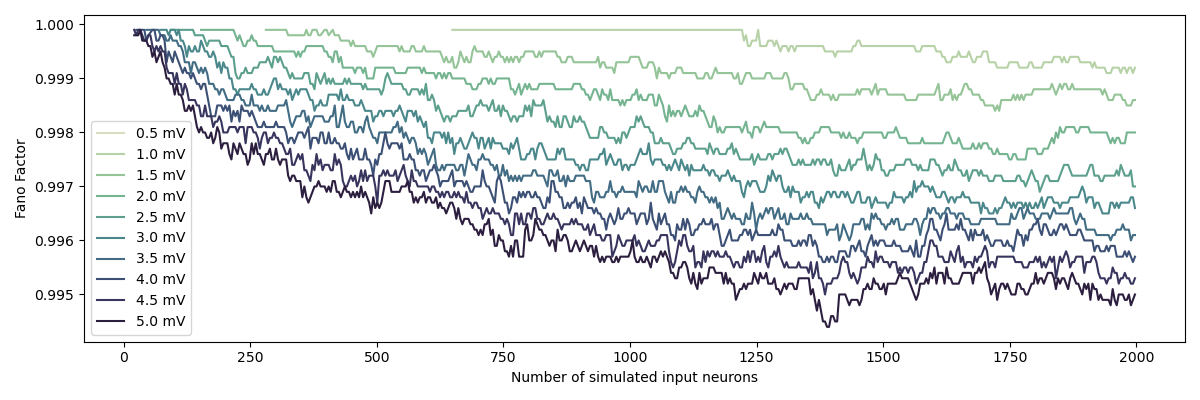
\includegraphics[width=1\linewidth]{Figure_FanoFactors.png}
    \caption{Fano factors difference calculated over different input neuron strengths and the number of input neurons based on the Poisson process}
    \label{fig:q3_graph2}
\end{figure}
There is a clear downward trend when the input strength is higher as well and the number of the simulated input neurons grows larger. Hence this shows a slight trend toward less variability relative to the mean spike count but the change is minimal, only 0.5\%. It is difficult to say if this difference is significant given its size, nonetheless, it can reflect some underlying model behaviour. 

I calculated the frequency change based on the ratio of the inhibitory and excitatory neuron inputs, from 1 inhibitory to 1000 excitatory input neurons, concretely from 1:1000 to 1000:1 number of excitatory to inhibitory Poisson process neuron inputs. From the simple graph \ref{fig:q3_graph3}, we can see the extreme importance of the inhibitory to excitatory input ratio as it has a large impact on the frequency of the firing rate of the simulated neuron. At first, with 1000 excitatory neurons the simulated neuron fired constantly however changing the ratio resulted in a seemingly linear decrease in the frequency, and slightly past the 1:1 ratio the frequency reached 0Hz. This suggests that at least for the simulated neuron, its characteristics of firing are largely dependent on its input ratio.

\begin{figure}[H]
    \centering
    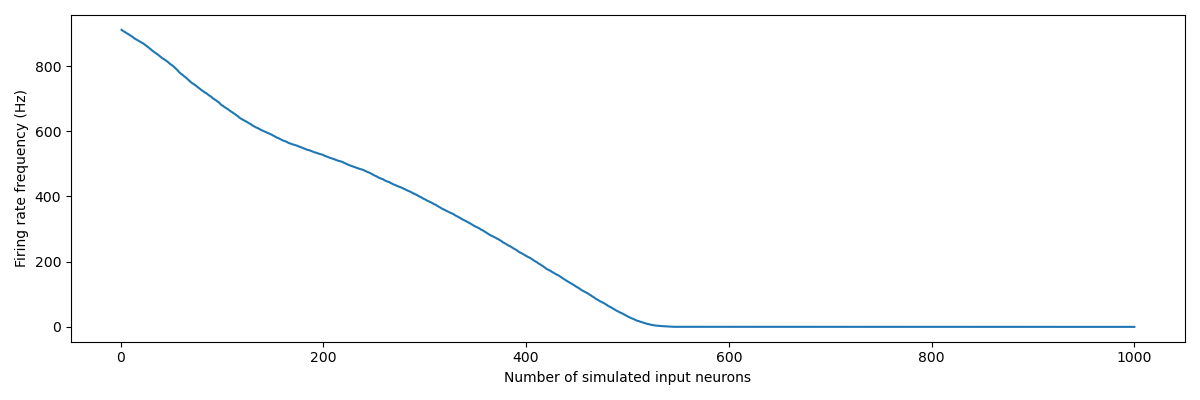
\includegraphics[width=0.83\linewidth]{Figure_ratio.png}
    \captionsetup{font=small}
    \caption{Frequency change based on a ratio between inhibitory and excitatory input neurons}
    \label{fig:q3_graph3}
\end{figure}

In the following graph\ref{fig:q3_graph4}, I plotted the calculated coefficients of variation from which we can see that when there is a smaller number of simulated input neurons the CV deviates from 1 frequently which shows the variability of the probabilistic nature of the input and when the number of those input neurons is smaller small deviations from the mean will make larger impact on the CV. Accordingly when the number of input neurons grows the closer they get to a CV value of 1. We can also observe that given small strength, we need more input neurons to trigger a spike in the integrate and fire neuron.\\
Further, it should also be noted that when changing the ratio between the inhibitory and excitatory input neurons the Fano factor remains close to 1.0, but with a high number of excitatory input neurons, its value is closer to 0.9 indicating some variability in spike counts. The coefficient of variation however was low, around 0.3 for a high number of excitatory input neurons but rises to one as we approach a 1 to 1 ratio after which it falls quickly due to inhibitory neurons causing fewer spikes up to a 0. The CV of 0.3 suggests a relatively regular firing pattern but not uniform but as we get closer to the 1 to 1 ratio the pattern becomes closer to a uniform distribution.

\begin{figure}[ht]
    \centering
    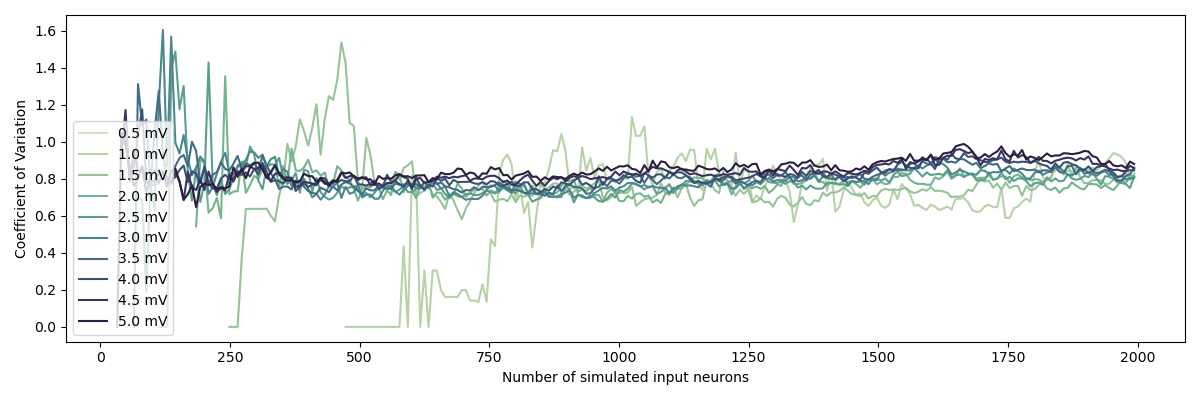
\includegraphics[width=1.0\linewidth]{Figure_CV.png}
    \captionsetup{font=small}
    \caption{Coefficient of variation}
    \label{fig:q3_graph4}
\end{figure}

\section*{Question 4} \label{question 4}
The spike-triggered average (STA) is given by $s(\tau) = \frac{1}{N} \sum_{i=1}^{N} p(t_i - \tau)$ for a neuron with spikes ${t_1,t_2,...,t_n}$ and the stimulus is $p(t)$.

\begin{wrapfigure}{l}{0.5\textwidth}
    \centering
    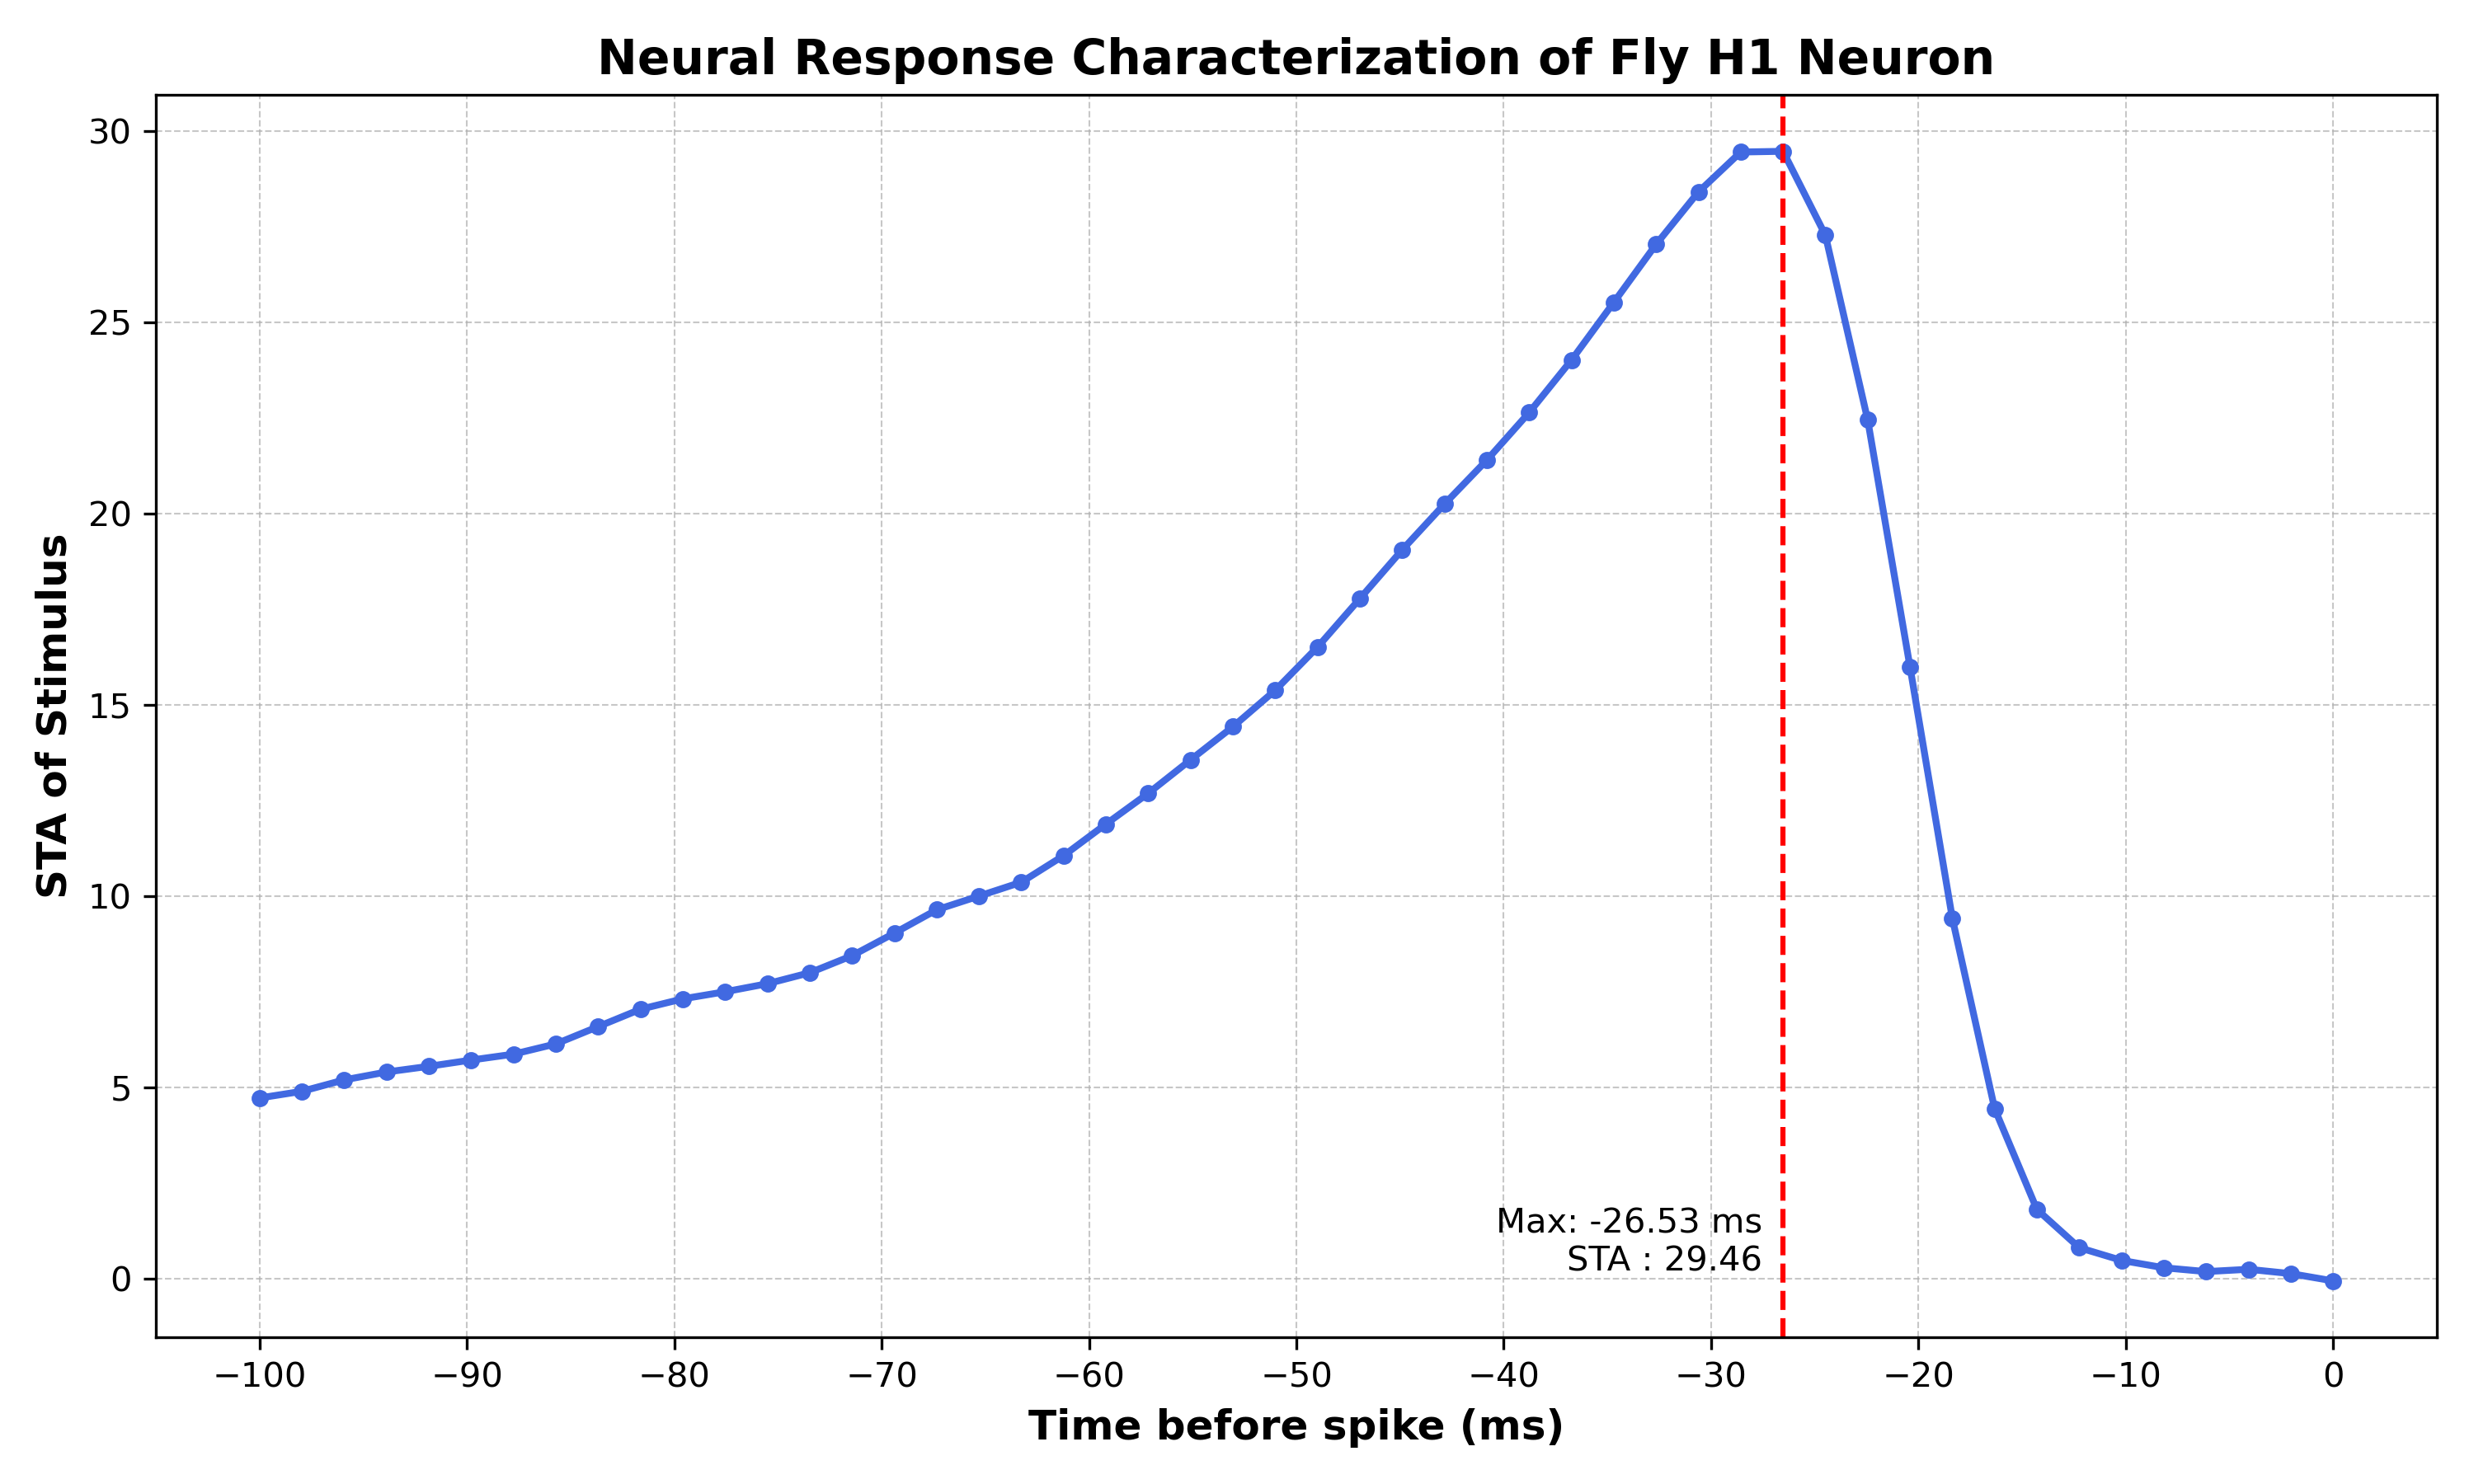
\includegraphics[width=1.0\linewidth]{Figure_STA.png}
    \caption{calculated STA over 100ms window from stimulus data in stim.dat and spike data in rho.dat}
    \label{fig:STAgraph1}
\end{wrapfigure}
The following graph \ref{fig:STAgraph1} shows the calculated STA over 100ms window for motion stimulus from the stim.dat file and the spike train from the rho.dat file that captures spikes of a fly H1 neuron. The graph suggests a specific pattern of stimulus before a spike is triggered. The curve's shape shows that there is a gradual increase in the stimulus up to about 26ms before a spike, with a sharp increase near the peak which is then followed by a steep decline in stimulus intensity just before the spike occurs, from 30ms before to spike. The shape indicates a specific stimuli input necessary for the spike to be triggered in a fly H1 neuron. This type of neuron is part of the fly's optic flow processing system and is particularly sensitive to horizontal motion across the visual field. The rise of the stimuli could represent a build-up of motion signals from the fly's visual field. The rapid decline could represent a cessation or rapid deceleration of motion in the visual field which could be critical for the fly to stabilise its flight or avoid obstacles. It could also show the neuron responds to the relative reduction in motion.


\section*{Question 5} \label{question 5}
The following graph \ref{fig:STAgraph2} shows the calculated values of the average stimulus before a pair of spikes that are in the intervals of 2ms, 10ms, 20ms, and 50ms for cases where the spikes are adjacent and non-adjacent, there are other spikes in between. It also combines the calculated STA for a single spike for comparison.

\begin{figure}[H]
    \centering
    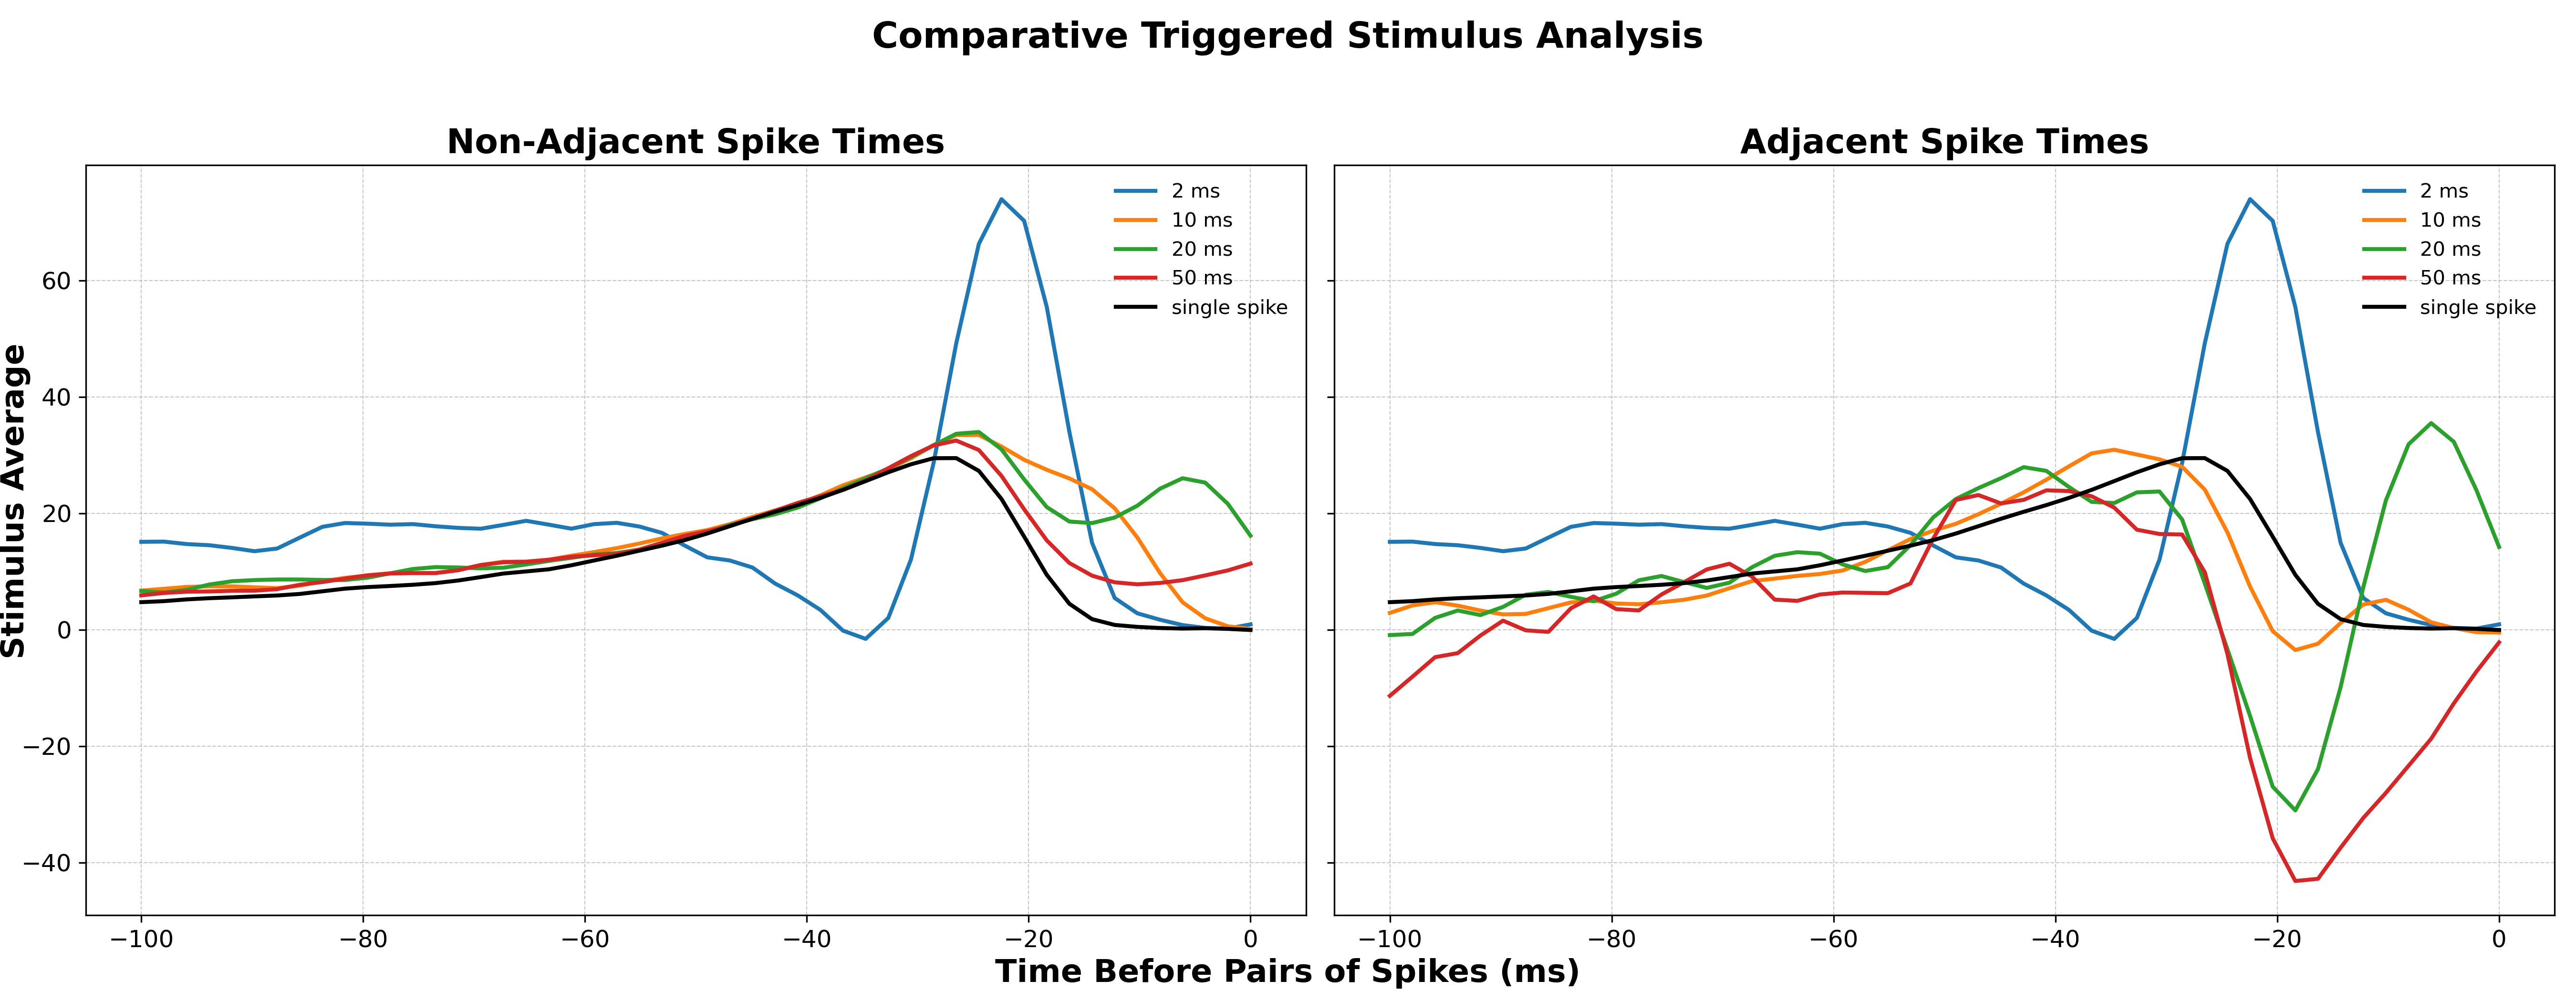
\includegraphics[width=1.0\linewidth]{Figure_STA_pairs.png}
    \caption{calculated STA over 100ms window from stimulus data in stim.dat and spike data in rho.dat}
    \label{fig:STAgraph2}
\end{figure}

There are significant differences between non-adjacent spikes and adjacent spikes, it should be noted that the calculated values for the 2ms interval are identical for both as the given 500Hz sampling rate only allows one measurement before another spike pair. Since this is a physical neuron it has a realistic refractory period between 2ms to 3ms meaning there cannot be another spike in the 2ms interval, hence the pairs in this case are identical.
For a pair of spikes in the 2ms interval, there is a specific stimuli curve especially between around 35ms and 5ms before the first pair of spikes. It increases sharply and decreases sharply at the same rate accounting for any measurement errors. This shows the neuron's high temporal resolution in response to rapid sensory input and shows it's tuned to detect and process rapid changes in the visual field.
For other intervals in the non-adjacent spike pairs, it is evident the amount of data that has been lost given the very strong influence of the STA of a single spike. To see the behaviour of the neuron for spike pairs it is therefore better to look at the graph with only adjacent pairs. Isolating the pairs from any other influence shows that using these different intervals, namely the 10ms, 20ms, and 50ms intervals, shows they are possibly similar. It can show how the H1 neuron encodes rapid motion information within the visual system of a fly and most notably shows bursty behaviour for rapidly increasing and then decreasing stimuli.

\section*{Question 6} \label{question 6}
To compare the flies H1 neuron to the simulated integrate and fire neuron I created a constant input of 10mV to be added to the stimulus and updated the neuron membrane potential as $R_mI$. The graph \ref{fig:STAgraph2} clearly shows a different behaviour for the simulated neuron. We can see the behaviour of the simulated neuron is much simpler and doesn't show any difference in pairs of spikes. This demonstrates the real H1 neuron is more complex and can model complex behaviour necessary for its function in the process of processing stimuli from the visual field. The integrate and fire model responds to the stimuli as expected given its simplicity, from the graph the neuron spikes when given a spiking stimuli input, the stimuli rise sharply over 30ms before triggering a spike.

\begin{figure}[H]
    \centering
    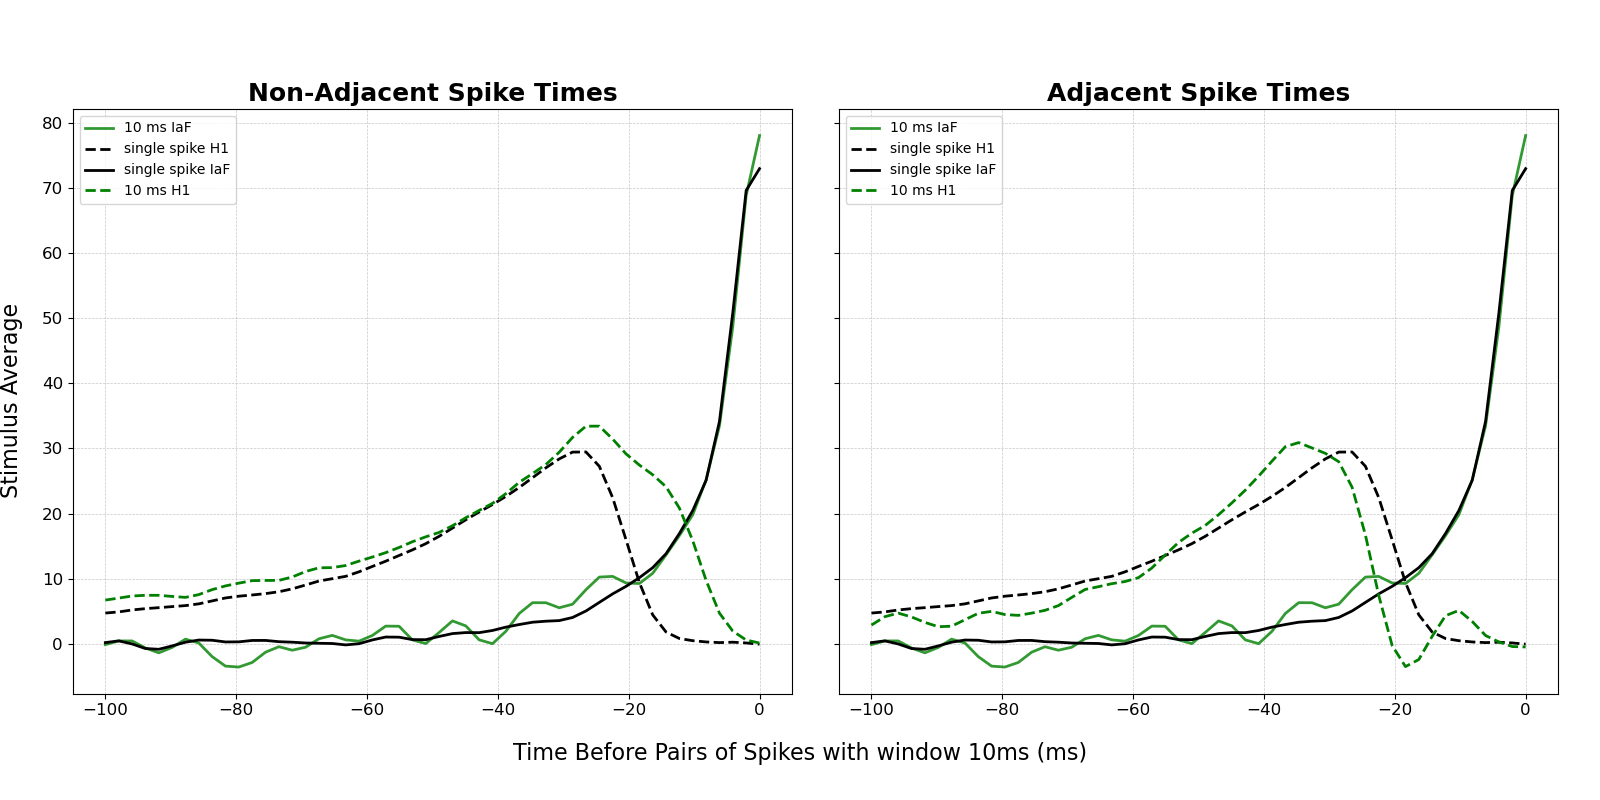
\includegraphics[width=1.0\linewidth]{Figure_STA_IaF.png}
    \captionsetup{font=small}
    \caption{The graph shows}
    \label{fig:STAgraph3}
\end{figure}

Next, I looked at the changes of the STA using the same stimulus but changing $\tau$, the membrane time constant to see its effects which are shown in graph \ref{fig:STAgraph3}.

\begin{figure}[H]
    \centering
    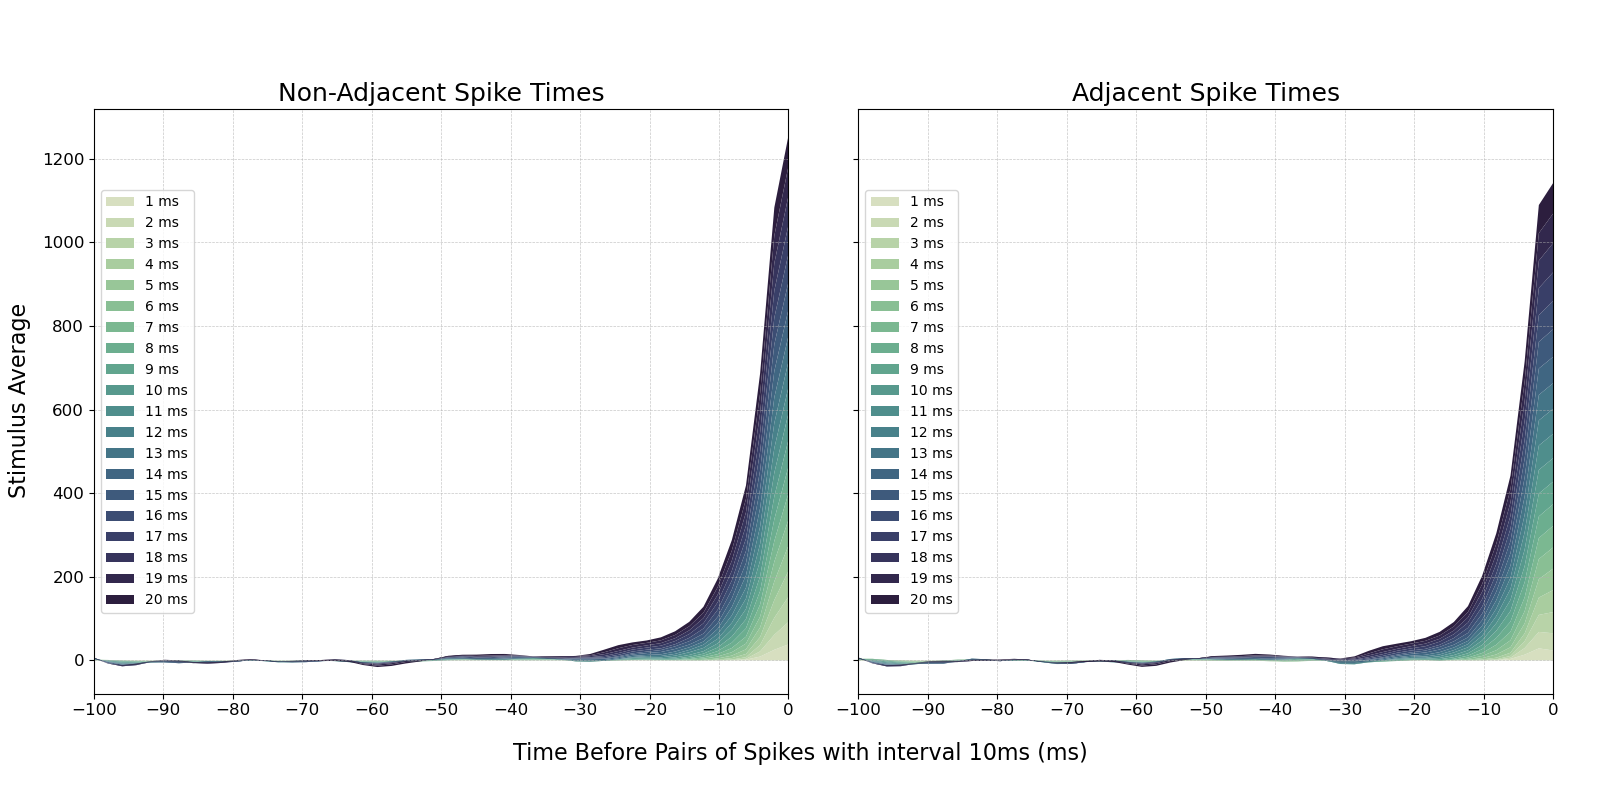
\includegraphics[width=0.99\linewidth]{Figure_tau_dependency.png}
    \caption{The graph shows}
    \label{fig:STAgraph3}
\end{figure}

Both graphs are expectedly almost identical, we can also clearly see that increasing the $\tau$ has quite significant influence over the stimuli triggering a spike. Irrespective of the value $\tau$, there is a clear spike in the values of stimuli before a spike, $\tau$ changes the onset of relevant stimuli as it needs longer to take effect. On the other hand, if the $\tau$ is small it needs only a few strong stimuli just before to spike, around 3 to 5 ms while a $\tau = 20 ms$ starts from 25 ms before the spike showing direct correlation with the membrane constant value. This simulation demonstrates that neurons with different membrane time constants respond differently to the same stimulus before spiking. This also affects the frequency of a neuron, smaller values of $\tau$ produce more bursty neurons or neurons of consistently higher fire rate.

\end{document}